\documentclass[a4paper,11pt]{exam}
%\printanswers % pour imprimer les réponses (corrigé)
\noprintanswers % Pour ne pas imprimer les réponses (énoncé)
\addpoints % Pour compter les points
% \noaddpoints % pour ne pas compter les points
%\qformat{\textbf{\thequestion ) } }
%\qformat{\textbf{\thequestion )}} % Pour définir le style des questions (facultatif)
\usepackage{color} % définit une nouvelle couleur
\shadedsolutions % définit le style des réponses
% \framedsolutions % définit le style des réponses
\definecolor{SolutionColor}{rgb}{0.8,0.9,1} % bleu ciel
\renewcommand{\solutiontitle}{\noindent\textbf{Solution:}\par\noindent} % Définit le titre des solutions




\makeatletter

\def\maketitle{{\centering%
	\par{\huge\textbf{\@title}}%
	\par{\@date}%
	\par}}


\renewcommand{\thesubsection}{\Alph{subsection}.}   

\makeatother

\lhead{NOM Pr\'enom :}
\rhead{\textbf{Les r\'eponses doivent \^etre justifi\'ees et r\'edig\'ees}}
\cfoot{\thepage / \pageref{LastPage}}


%\usepackage{../../pas-math}
%\usepackage{../../moncours}


%\usepackage{pas-cours}
%-------------------------------------------------------------------------------
%          -Packages nécessaires pour écrire en Français et en UTF8-
%-------------------------------------------------------------------------------
\usepackage[utf8]{inputenc}
\usepackage[frenchb]{babel}
%\usepackage{numprint}
\usepackage[T1]{fontenc}
%\usepackage{lmodern}
\usepackage{textcomp}
\usepackage[french, boxed]{algorithm2e}
\usepackage{hyperref}


%-------------------------------------------------------------------------------

%-------------------------------------------------------------------------------
%                          -Outils de mise en forme-
%-------------------------------------------------------------------------------
\usepackage{hyperref}
\hypersetup{pdfstartview=XYZ}
%\usepackage{enumerate}
\usepackage{graphicx}
\usepackage{multicol}
\usepackage{tabularx}
\usepackage{multirow}
\usepackage{color}
\usepackage{eurosym}


\usepackage{anysize} %%pour pouvoir mettre les marges qu'on veut
%\marginsize{2.5cm}{2.5cm}{2.5cm}{2.5cm}

\usepackage{indentfirst} %%pour que les premier paragraphes soient aussi indentés
\usepackage{verbatim}
\usepackage{enumitem}
\usepackage{booktabs}
\usepackage[usenames,dvipsnames,svgnames,table]{xcolor}

\usepackage{variations}

%-------------------------------------------------------------------------------


%-------------------------------------------------------------------------------
%                  -Nécessaires pour écrire des mathématiques-
%-------------------------------------------------------------------------------
\usepackage{amsfonts}
\usepackage{amssymb}
\usepackage{amsmath}
\usepackage{amsthm}
\usepackage{tikz}
\usepackage{xlop}
\usepackage[output-decimal-marker={,}]{siunitx}
%-------------------------------------------------------------------------------

%-------------------------------------------------------------------------------
%                  -Nécessaires pour écrire des formules chimiquess-
%-------------------------------------------------------------------------------

\usepackage[version=4]{mhchem}

%-------------------------------------------------------------------------------
% Pour pouvoir exploiter les fichiers directement dans beamer
\newcommand{\pause}{\ }
%-------------------------------------------------------------------------------
%                    - Mise en forme avancée
%-------------------------------------------------------------------------------

\usepackage{ifthen}
\usepackage{ifmtarg}


\newcommand{\ifTrue}[2]{\ifthenelse{\equal{#1}{true}}{#2}{$\qquad \qquad$}}

%\newcommand{\kword}[1]{\textcolor{red}{\underline{#1}}}
%-------------------------------------------------------------------------------

%-------------------------------------------------------------------------------
%                     -Mise en forme d'exercices-
%-------------------------------------------------------------------------------
%\newtheoremstyle{exostyle}
%{\topsep}% espace avant
%{\topsep}% espace apres
%{}% Police utilisee par le style de thm
%{}% Indentation (vide = aucune, \parindent = indentation paragraphe)
%{\bfseries}% Police du titre de thm
%{.}% Signe de ponctuation apres le titre du thm
%{ }% Espace apres le titre du thm (\newline = linebreak)
%{\thmname{#1}\thmnumber{ #2}\thmnote{. \normalfont{\textit{#3}}}}% composants du titre du thm : \thmname = nom du thm, \thmnumber = numéro du thm, \thmnote = sous-titre du thm

%\theoremstyle{exostyle}
%\newtheorem{exercice}{Exercice}
%
%\newenvironment{questions}{
%\begin{enumerate}[\hspace{12pt}\bfseries\itshape a.]}{\end{enumerate}
%} %mettre un 1 à la place du a si on veut des numéros au lieu de lettres pour les questions 
%-------------------------------------------------------------------------------

%-------------------------------------------------------------------------------
%                    - Mise en forme de tableaux -
%-------------------------------------------------------------------------------

\renewcommand{\arraystretch}{1.7}

\setlength{\tabcolsep}{1.2cm}

%-------------------------------------------------------------------------------



%-------------------------------------------------------------------------------
%                    - Racourcis d'écriture -
%-------------------------------------------------------------------------------
%Droites
\newcommand{\dte}[1]{$(#1)$}
\newcommand{\fig}[1]{figure $#1$}
\newcommand{\sym}{symétrique}
\newcommand{\syms}{symétriques}
\newcommand{\asym}{axe de symétrie}
\newcommand{\asyms}{axes de symétrie}
\newcommand{\seg}[1]{$[#1]$}
\newcommand{\monAngle}[1]{$\widehat{#1}$}
\newcommand{\bissec}{bissectrice}
\newcommand{\mediat}{médiatrice}
\newcommand{\ddte}[1]{$[#1)$}


% Angles orientés (couples de vecteurs)
\newcommand{\aopp}[2]{(\vec{#1}, \vec{#2})} %Les deuc vecteurs sont positifs
\newcommand{\aopn}[2]{(\vec{#1}, -\vec{#2})} %Le second vecteur est négatif
\newcommand{\aonp}[2]{(-\vec{#1}, \vec{#2})} %Le premier vecteur est négatif
\newcommand{\aonn}[2]{(-\vec{#1}, -\vec{#2})} %Les deux vecteurs sont négatifs

%Ensembles mathématiques
\newcommand{\naturels}{\mathbb{N}} %Nombres naturels
\newcommand{\relatifs}{\mathbb{Z}} %Nombres relatifs
\newcommand{\rationnels}{\mathbb{Q}} %Nombres rationnels
\newcommand{\reels}{\mathbb{R}} %Nombres réels
\newcommand{\complexes}{\mathbb{C}} %Nombres complexes


%Intégration des parenthèses aux cosinus
\newcommand{\cosP}[1]{\cos\left(#1\right)}
\newcommand{\sinP}[1]{\sin\left(#1\right)}


%Probas stats
\newcommand{\stat}{statistique}
\newcommand{\stats}{statistiques}


\newcommand{\homo}{homothétie}
\newcommand{\homos}{homothéties}


\newcommand{\mycoord}[3]{(\textcolor{red}{\num{#1}} ; \textcolor{Green}{\num{#2}} ; \textcolor{blue}{\num{#3}})}
%-------------------------------------------------------------------------------

%-------------------------------------------------------------------------------
%                    - Mise en page -
%-------------------------------------------------------------------------------

\newcommand{\twoCol}[1]{\begin{multicols}{2}#1\end{multicols}}


\setenumerate[1]{font=\bfseries,label=\textit{\alph*})}
\setenumerate[2]{font=\bfseries,label=\arabic*)}


%-------------------------------------------------------------------------------
%                    - Elements cours -
%-------------------------------------------------------------------------------

%Correction d'exercice
\newcommand{\exoSec}[2]{\subsection*{Exercice #1 page #2}}
%-------------------------------------------------------------------------------
%                    - raccourcis d'écriture -
%-------------------------------------------------------------------------------

%Mise en évidence de termes clés
\newcommand{\mykw}[1]{\textcolor{red}{\underline{\textbf{#1}}}}

%Exercices
\newcommand{\exo}[2]{exercice #1 page #2}
\newcommand{\Exo}[2]{Exercice #1 page #2}

\renewcommand{\pause}{\ }

%Intervalles
\newcommand{\interOO}[2]{$]$#1 , #2$[$}
\newcommand{\interOF}[2]{$]$#1 , #2$]$}
\newcommand{\interFO}[2]{$[$#1 , #2$[$}
\newcommand{\interFF}[2]{$[$#1 , #2$]$}



%\usepackage{fullpage}
\author{\ }
\date{21 Mars 2018}
\title{Sciences Physiques : DS n° 5}


\begin{document}
%	\usepackage{fancyhdr}
%	
%	\pagestyle{fancy}
%	\fancyhf{}
	%\rhead{Share\LaTeX}


	\maketitle


\begin{small}
	\begin{center}
		\begin{tabular}{|@{\ }l@{}|@{\ }c@{\ }|}
			\hline
			\textbf{Compétence} & \textbf{Maitrise} \\
			\hline
			Caractériser le mouvement d’un objet \ \ &  \ \ \ \\
			\hline
			Mouvements rectilignes et circulaires. &  \\
			\hline			
			Relativité du mouvement dans des cas simples.  \ \  &  \\
			\hline
			
		\end{tabular}
	\end{center}
\end{small}	
\vspace*{-0.5cm}	

\section{QCM (3 points)}

Pour chaque question, choisir la (ou les) bonnes réponses

\begin{questions}
	
	\begin{multicols}{2}
		
		\question[\half] Le ballon de handball est en mouvement par rapport :
	
	
	
		
	\begin{checkboxes}
		\correctchoice au sol.
		\correctchoice à un joueur.
		\choice au ballon.
	\end{checkboxes}

	\begin{center}
		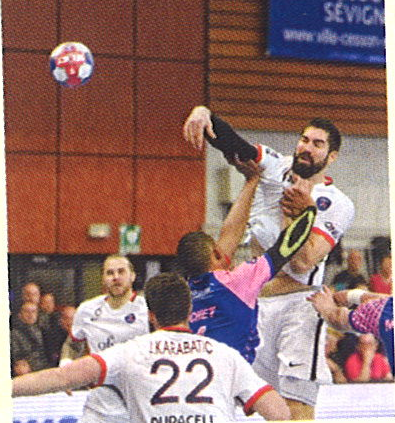
\includegraphics[scale=0.3]{hand}
	\end{center}
	\end{multicols}

	\question[\half] La tour Eiffel est fixe par rapport :\\
	\begin{oneparcheckboxes}
		\choice à la Lune.
		\correctchoice à la surface de la Terre.
		\choice au Soleil
	\end{oneparcheckboxes}

	\question[\half] Les passagers d'une grande roue pendant son fonctionnement sont immobiles par rapport :
	\begin{oneparcheckboxes}
		\correctchoice à leur nacelle.
		\choice au sol.
		\choice au centre de la roue.
	\end{oneparcheckboxes}



	\begin{multicols}{2}
		\question[\half] L'image ci-dessous est une chronophotographie d'un saut en bmx. La trajectoire du casque par rapport au sol est :
	\begin{checkboxes}
		\correctchoice curviligne.
		\choice rectiligne.
		\choice circulaire.
	\end{checkboxes}

	
	\begin{center}
		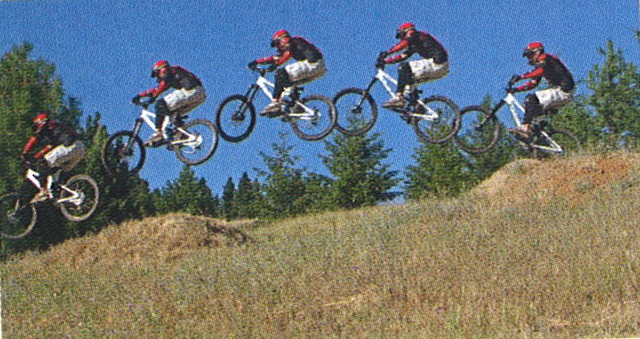
\includegraphics[scale=0.3]{bmx}
	\end{center}

	\end{multicols}
	\question[\half] La trajectoire de la nacelle d'une grande roue par rapport au sol est :\\
	\begin{oneparcheckboxes}
		\choice curviligne.
		\choice rectiligne.
		\correctchoice circulaire.
	\end{oneparcheckboxes}
	
	
	\begin{multicols}{2}
		\question[\half] La trajectoire du casque par rapport au centre de la Terre de ces enfants assis sur un banc est :
	\begin{checkboxes}
		\choice curviligne.
		\choice rectiligne.
		\correctchoice circulaire.
	\end{checkboxes}

	\begin{center}
		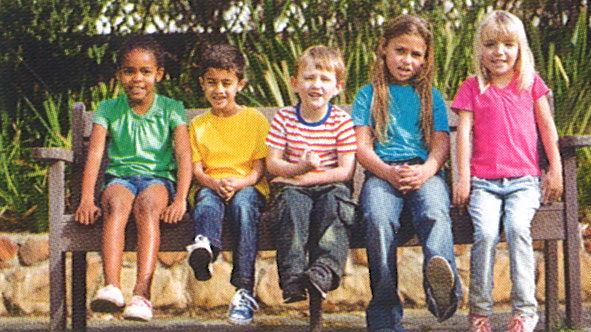
\includegraphics[scale=0.3]{banc}
	\end{center}
	\end{multicols}
\end{questions}



%\newpage

\section{Déterminer un référentiel (4 points)}

\begin{center}
	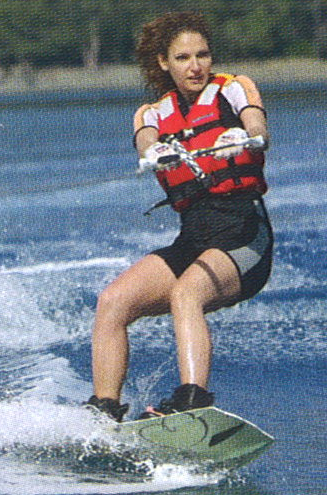
\includegraphics[scale=0.3]{board}
\end{center}

Un bateau se déplace sur un plan d'eau en ligne droite à une vitesse constante.
La wakeboardeuse, tractée par ce bateau a la même trajectoire.
\begin{questions}
	\question Déterminer dans quel référentiel la wakeboardeuse est :
	
	\begin{parts}
		\part[2] immobile
		\fillwithdottedlines{3cm}
		\part[2] en mouvement
		\fillwithdottedlines{3cm}
	\end{parts}
\end{questions}

\section{Désigner un référentiel (3 points)}
\begin{questions}
	
\question[3] Dans quel référentiel, parmi ceux proposés ci-dessous, a personne sur le tapis roulant en fonctionnement est-elle immobile ?
 
\end{questions}

\begin{multicols}{2}
	 
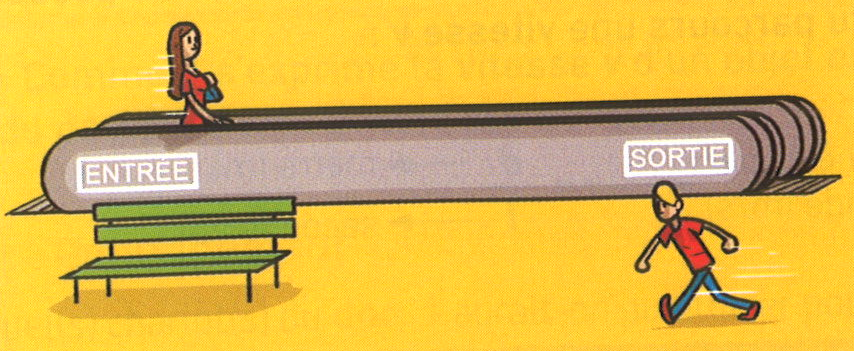
\includegraphics[scale=0.3]{tapis}
 
 \begin{enumerate}
 	\item Le tapis roulant.
 	\item La personne qui marche à l'extérieur du tapis roulant.
 	\item La banc. 
 \end{enumerate}



\end{multicols}
\fillwithdottedlines{3.5cm}
\newpage 
\section{Une grue de chantier (3 points)}

Les grues permettent de soulever et de déplacer les charges les plus lourdes présentent sur un chantier.

\begin{questions}
	\question[3] Quels types de mouvements la charge transportée peut-elle avoir lorsqu'elle est au bout du câble ? Expliquer les réponses.
\end{questions}

\fillwithdottedlines{5cm}


\section{Trombone à coulisse}

Pour jouer ses notes, le tromboniste utilise une coulisse qu'il descend ou remonte avec la main droite, ce qui allonge ou raccourcit le trajet de l'air qu'il souffle.

\begin{questions}
	\question Que peut-on dire du mouvement de la coulisse ?
	
	\fillwithdottedlines{3cm}
	
	\question Dans le fonctionnement d'un violon, quelle pièce aura un mouvement du même type.
	\fillwithdottedlines{3cm}
\end{questions}

\newpage

\section{La bonne trajectoire (3 points)}

\begin{questions}
	\begin{multicols}{2}
		\question[3] Décrire la trajectoire de la voiture entre les points : 
	\begin{itemize}
		\item A et B
		\item B et C
		\item C et D
	\end{itemize}

	\begin{center}
		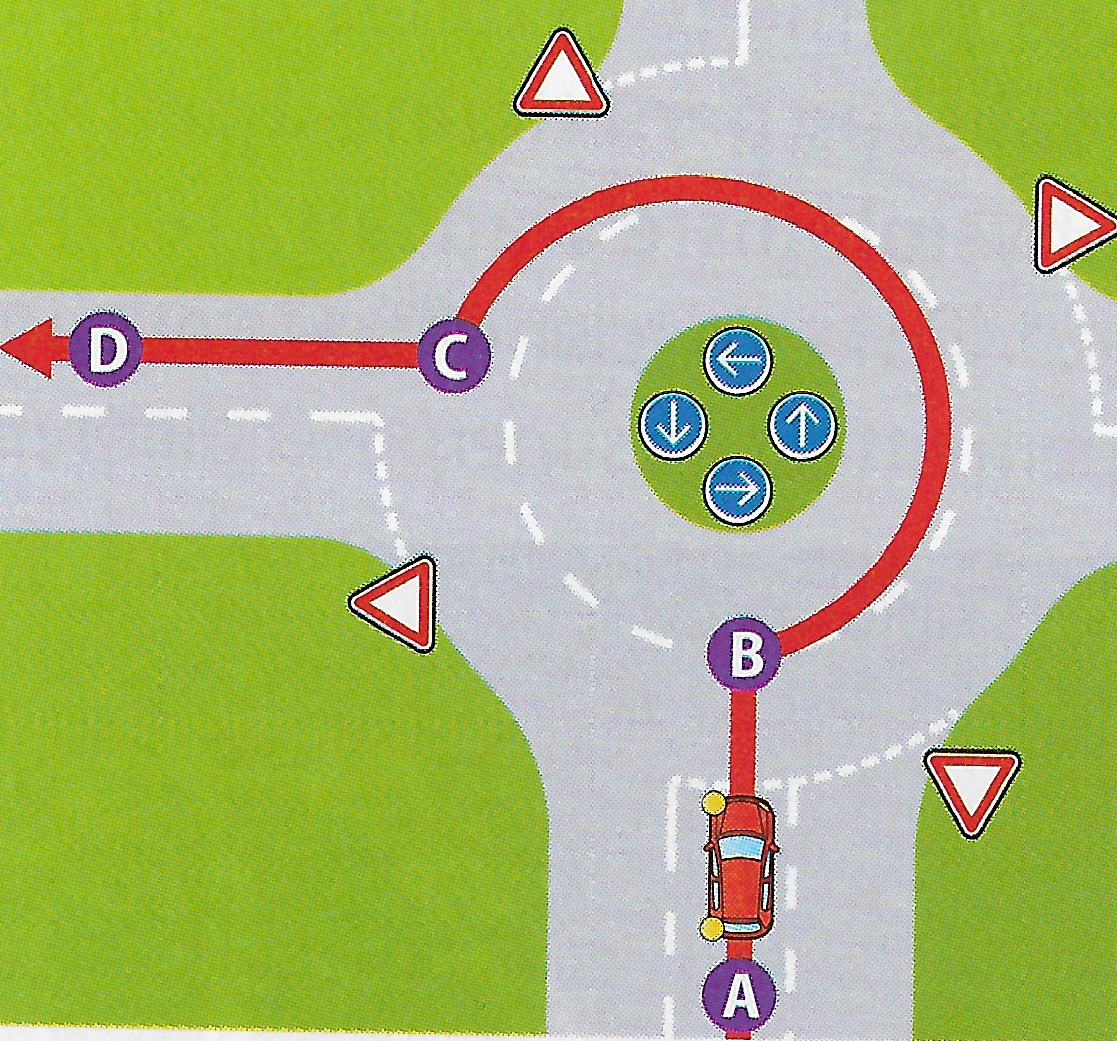
\includegraphics[scale=1]{rp}
	\end{center}
	\end{multicols}

	\fillwithdottedlines{4cm}
\end{questions}



\ \label{LastPage}

\end{document}